\Chapter{Tesztelés}

5 város esetén
Összehasonlítások száma: 74 434
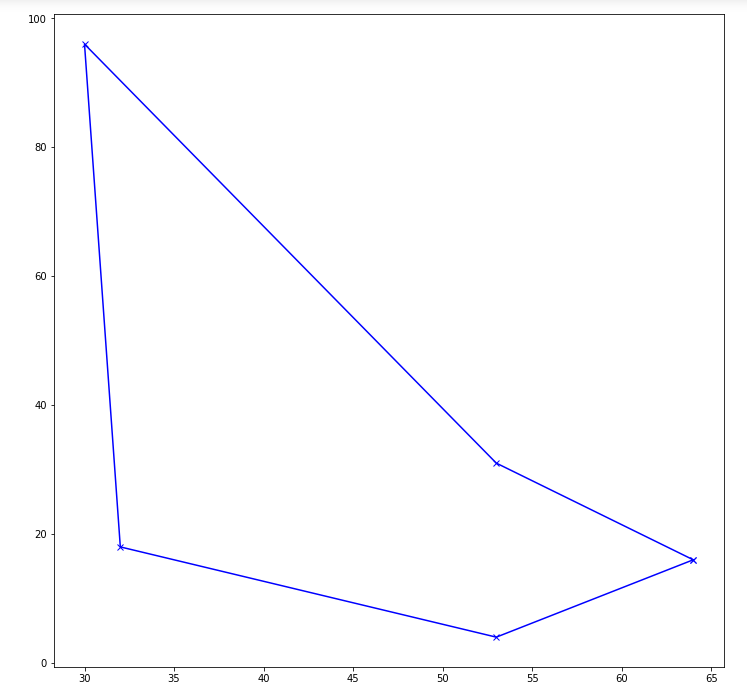
\includegraphics[scale=0.4]{images/5.png}

10 város esetén
Összehasonlítások száma: 68 594
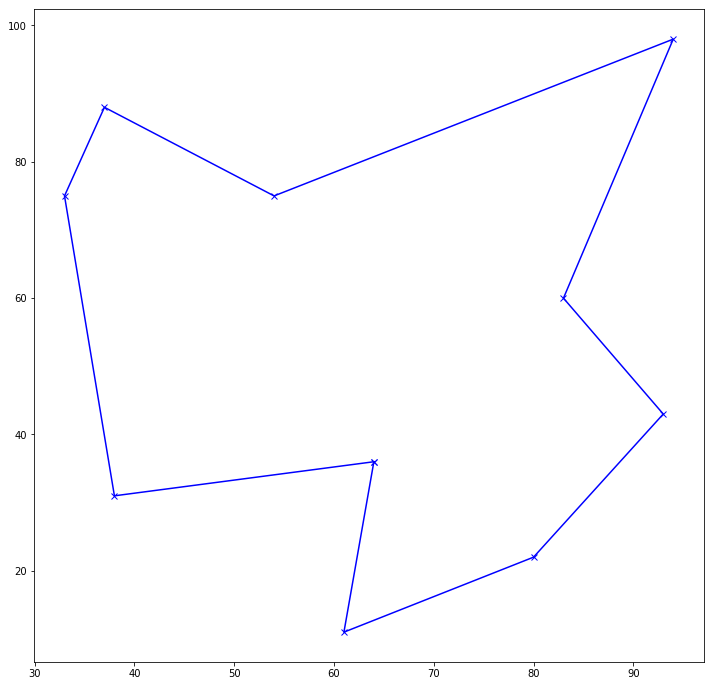
\includegraphics[scale=0.4]{images/10.png}

15 város esetén
Összehasonlítások száma: 66 672
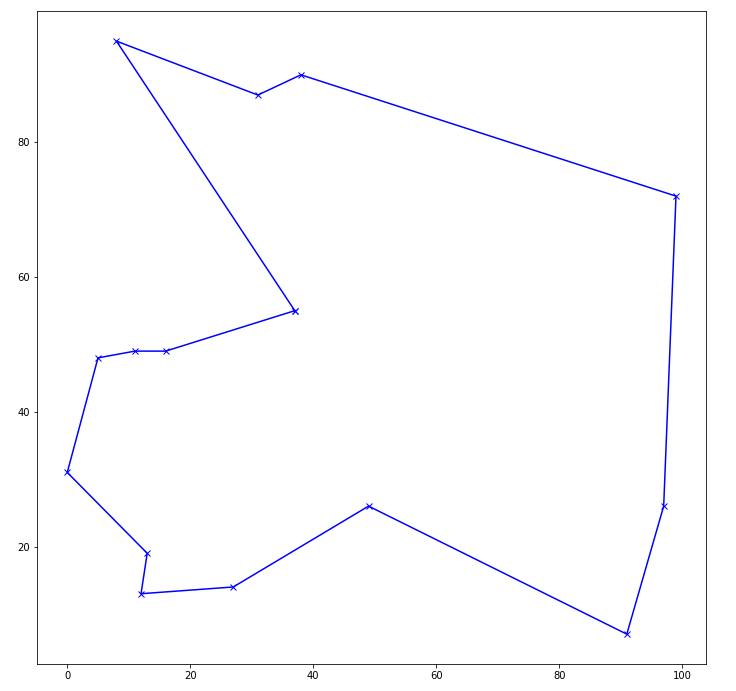
\includegraphics[scale=0.4]{images/15.png}

20 város esetén
Összehasonlítások száma: 65 265
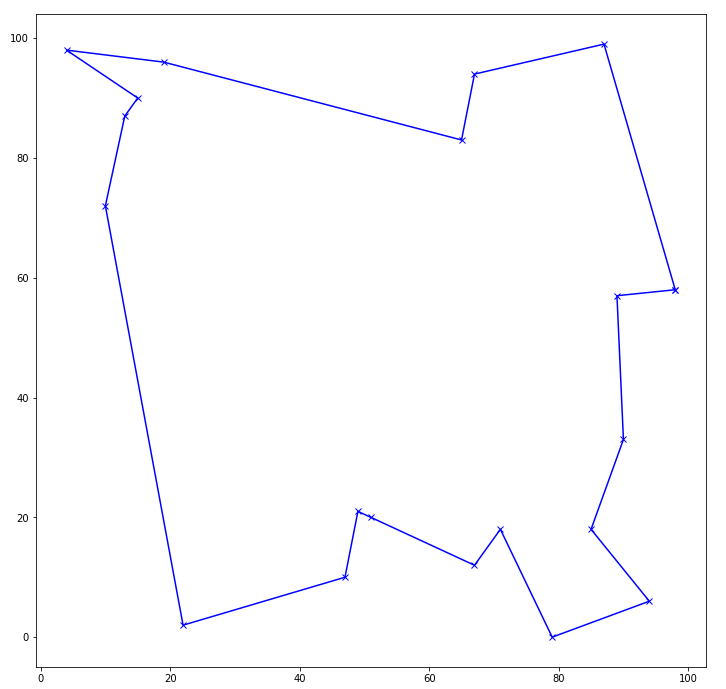
\includegraphics[scale=0.4]{images/20.png}

25 város esetén
Összehasonlítások száma: 67 865
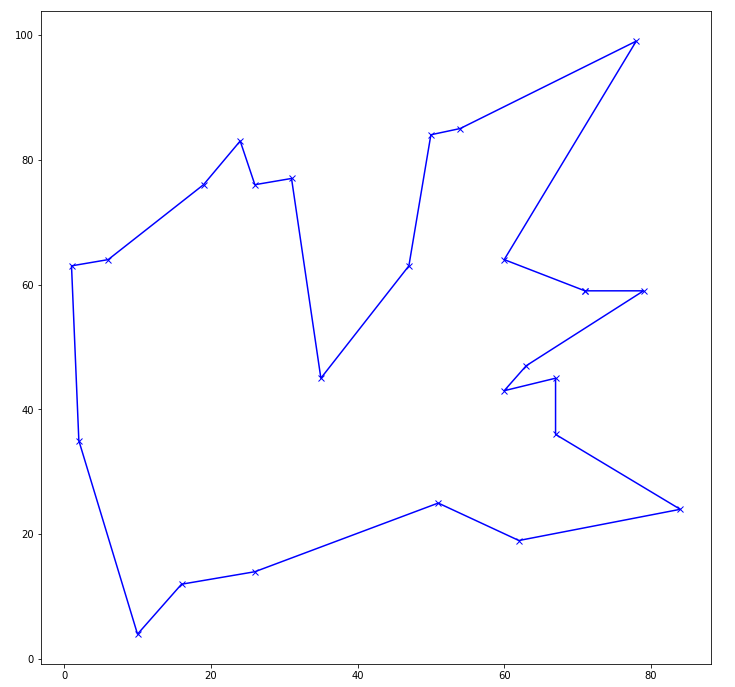
\includegraphics[scale=0.4]{images/25.png}

30 város esetén
Összehasonlítások száma: 65 324
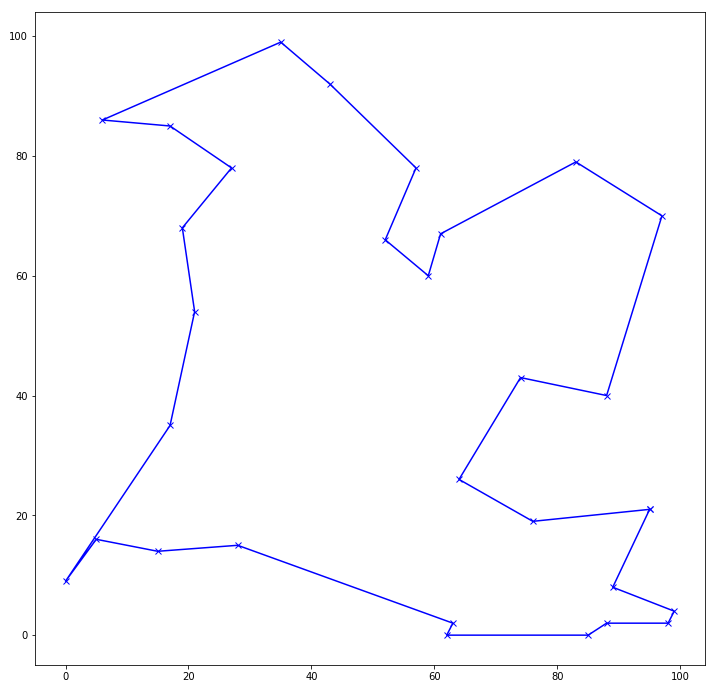
\includegraphics[scale=0.4]{images/30.png}

35 város esetén
Összehasonlítások száma: 67 230
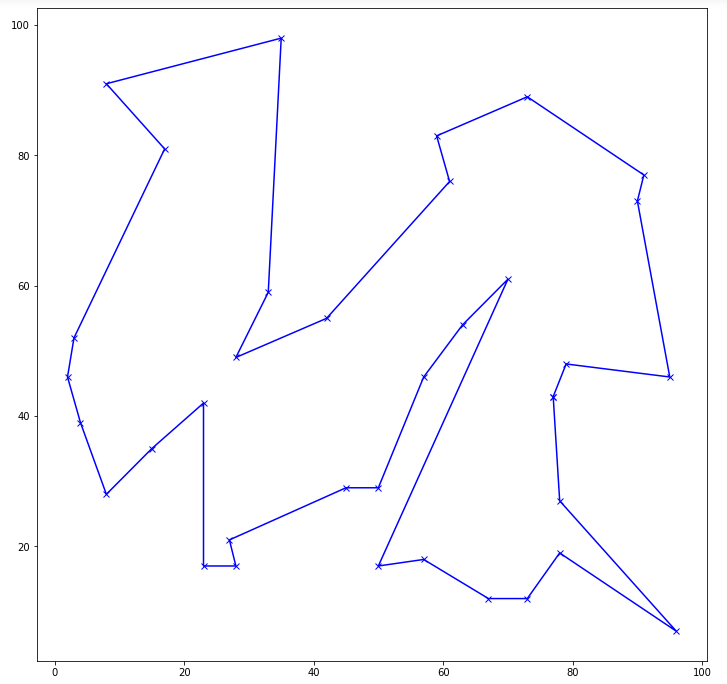
\includegraphics[scale=0.4]{images/35.png}

40 város esetén
Összehasonlítások száma: 66 008
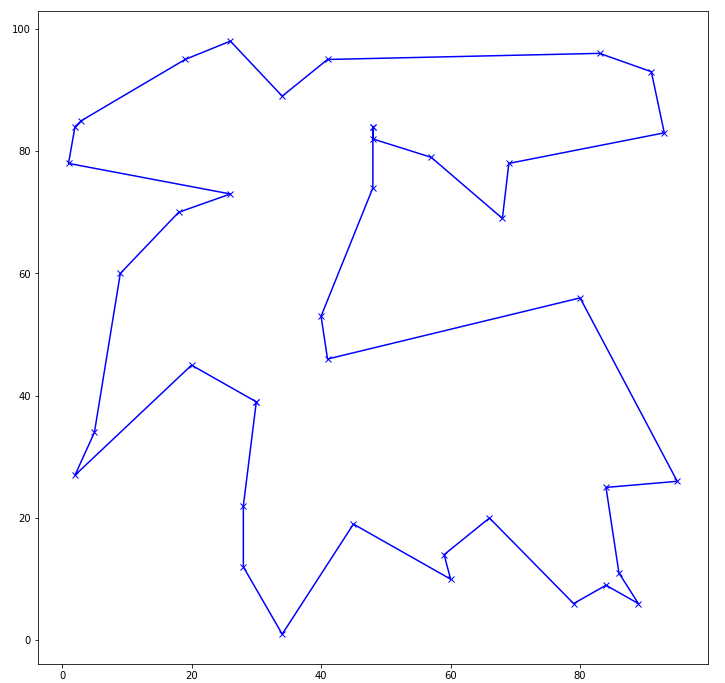
\includegraphics[scale=0.4]{images/40.png}


Több lefuttatott teszt után is megfgyelhető, hogy az összehasonlítások száma 65 ezer és 75 ezer között mozog. Egytől egyig az optimális utat adták.

A következő gráfok megmutatják a kívánt utat vároksok száma szerint. Mivel véletlenszerű számok összehasonlításán alapszik az algoritmus ezáltal az összehasonlítások száma igen magas, viszont stagnál bizonyos értékek között.
